\documentclass{stdlocal}
\begin{document}
\section{Implementation} % (fold)
\label{sec:implementation}
  In the section \ref{sec:pseudorandom_number_generators}, we have already discussed the mathematical foundations of PRNGs, as well as some examples, like the MT19937.
  In this section, we will first implement a scalar variant of the chosen generators to better understand their structure and design.
  Moreover, they serve as a testing facility to make sure the output of the vectorized PRNGs is correct.
  After explaining the critical points in the implementation, we will show how to vectorize the given generators.
  For this, it is helpful to first discuss which technique to use for the vectorization.
  Afterwards a theoretical analysis of the used vector intrinsics concerning their latency and throughput will follow to pinpoint bottlenecks of the implementation possibly resulting in future work.

  \subsection{MT19937} % (fold)
  \label{sub:mersenne_twister}
    The MT19937 is de facto standard of applications using random numbers to compute their results.
    In the original paper, \citeauthor{matsumoto1998} have given a standard implementation in the C programming language.
    This implementation is easily adjustable to work in C++.
    To map the C-style functional programming to modern C++ paradigms, we introduce a functor that stores the complete state of the Mersenne Twister.
    The functional operator is then used to represent the application of the transition and generator function to receive a new random number.
    The introduction of the functor grants us the complete power of the C++ template, type, and class system while preserving an easy-to-use interface.

    In \textcite{kneusel2018}, a special seeding routine was used, such that the actual initialization process only needs one truly random number.
    In the STL of the C++ programming language the MT19937 is already implemented.
    The corresponding class is called \code{std::mt19937} and offers a constructor with only one integral number of $32\appendUnit{bit}$ length as seeding value.
    This constructor uses the initialization routine described by \textcite{kneusel2018}.
    We want to make sure, that our implementation gives exactly the same output as the standard variant while keeping the advantages of our own API.
    As a consequence, we have to introduce a structure which can be interpreted as a PRNG and should serve as a default seeder for the MT19937.

    Additionally, the types and parameters of the MT19937 will be defined as compile-time constants inside the functor to make sure the code stays maintainable by not inserting magic numbers in the implementation.
    To guarantee that there is no runtime overhead, we defined those variables as \code{static constexpr}.

    \inputCodeBlock[title = Scalar MT19937 Structure]{code/mt19937/sisd/struct.hpp}
    Implementing the default seeder is done the same way as the MT19937 itself.
    First, we introduce a functor with the appropriate state while using the function operator as advancing routine.
    The initialization from \textcite{kneusel2018} was slightly changed to adapt to the new functor definitions.
    By designing a fast-forward constructor, it is possible to seed our own MT19937 with any other RNG including the default seeder.

    \inputCodeBlock[title = Scalar MT19937 Seeding]{code/mt19937/sisd/seeding.hpp}
    Advancing the state of the MT19937 by asking for a random number is a more complicated algorithm.
    The recurrence of the Mersenne Twister is linear and gives us an equation on how to get to the next element based on the $624$ current elements.
    According to the mathematics, after the computation we would have to move every element of the state one step further.
    But accessing each element in the state vector for every random number would greatly reduce the performance due to cache misses and the time to move every element.
    Instead, \citeauthor{matsumoto1998} cache the index of the current element in the state.
    While the cached index is small enough, advancing the state only results in incrementing the index and returning the state value at this position by applying the generator function.
    Only if the index reaches the end of the state vector the complete state vector will be regenerated with respect to the recursive relation.
    In our code, the regeneration of the state vector uses a lambda expression to reduce code duplication and improve code transparency.
    The lambda expression keeps the code local in contrast to helper or member function.
    Hence, the compiler will probably inline all calls to the lambda expression optimizing the scalar code in the best possible way.

    \begin{figure}
      \center
      \begin{subfigure}[b]{0.3\textwidth}
        \center
        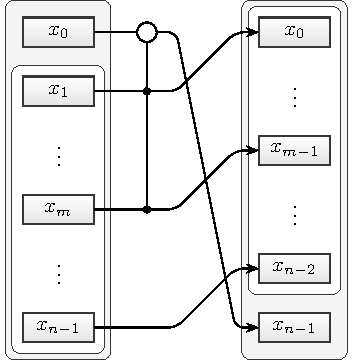
\includegraphics[width=0.95\textwidth]{figures/mt19937_transition_short.pdf}
      \end{subfigure}
      \begin{subfigure}[b]{0.68\textwidth}
        \center
        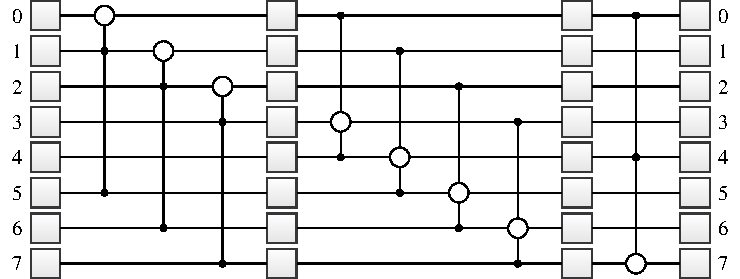
\includegraphics[width=0.95\textwidth]{figures/mt19937_loop_scheme.pdf}
      \end{subfigure}
      \caption[Mersenne Twister Loop Scheme]{}
      \label{fig:mt-loop-scheme}
    \end{figure}

    \begin{figure}
      \center
      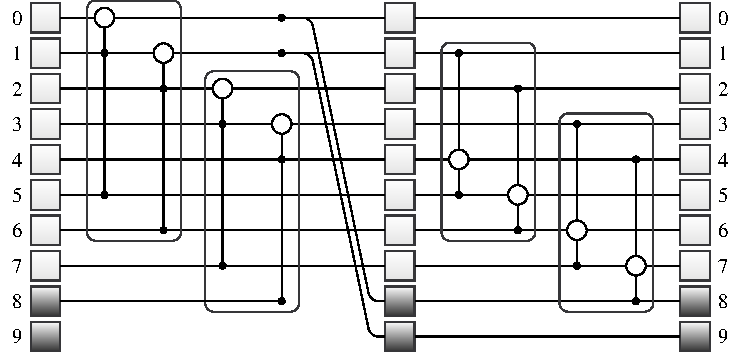
\includegraphics[width=0.95\textwidth]{figures/mt19937_vector_loop_scheme.pdf}
      \caption[Mersenne Twister Vector Loop Scheme]{}
      \label{fig:mt-vector-loop-scheme}
    \end{figure}

    \inputCodeBlock[title = Scalar MT19937 Advancing]{code/mt19937/sisd/advance.hpp}
    The design of our Mersenne Twister ensures that the output will be the same as the output of the MT19937 from the STL of the C++ programming language.
    Additionally, the interface provides a more general seeding variant which improves statistical performance for seeding generators other than the default seeder.
    The new initialization facility is easier to use and gives a better {}insight into the used seeding values to the reader of the code.
    The function to advance the state is easier to understand, maintainable and generalizable.
    Last but not least, as we will show, our MT19937 implementation is able to provide a better performance in an actual application.

    Because the state of the MT19937 is very large in comparison to the size of the SSE and AVX vector registers, we rely on a typical vectorization technique described by \textcite{fog2015} that does not need to initialize multiple instances of the same generator.
    The scalar implementation offers a large degree of data independence.
    After the regeneration of the complete state vector, the generator function has to be applied on each individual element to provide random numbers.
    This problem describes the perfect use case for SIMD intrinsics.
    In the AVX case, we can read eight $32\appendUnit{bit}$ values at the same time by the usage of a vector register and apply the generator function on each element in parallel by using the respective intrinsics.
    In the SSE case, we would only read four elements.
    The number of elements in the state vector is divisible by the eight and four without remainder.
    Hence, we do not have to take care of the boundaries of the state vector.

    The moment every package of eight or four elements in the state vector was read, the regeneration has to be triggered.
    The computation of the new state vector exhibits some data dependencies we have to take care of.
    In the scalar variant of the regeneration process the loop of all elements was split into three parts --- one for the first $227$ elements, one for the following $396$ elements and one for the last element.
    The splitting followed from the dependencies given by the recurrence defining the Mersenne Twister algorithm.
    All elements in the first loop have to access the elements at the same position, one position ahead and $397$ steps ahead.
    Reaching the $227$.~element will then forbid us to go $397$ steps further, because the position would not lie inside the state vector.
    But the requested element has already been produced at position zero.
    Therefore all elements in the second loop need to access the elements at the same position, one position ahead and $227$ steps backwards.
    For the last element the successive element would again lie outside the state vector.
    Hence, the last elements uses the elements at the last position and positions zero and $396$.

    Thus all newly generated elements in the first loop are independent of each other and can therefore be vectorized.
    This is also true for the second loop after the first loop has been executed.
    The problem lies in the fact that the number $397$, as well as $227$, is not divisible by eight or four without remainder.
    This leads to the appearance of a boundary vector term for the last element at the end of the state vector and one between the first and the second loop which needs to access successive and previous elements at the same time.
    Handling these boundary terms explicitly through vector intrinsics will result in complex loading, storing and blend operations.
    We have chosen another path by slightly changing the layout of the underlying data structure.
    Instead of saving only $624$ elements for the state vector, we append values at the end of the state vector to get a buffer that should reduce complexity.
    The number of values we append is given by the amount of elements that fit into a vector register.
    After the generation of the first vector unit in the first loop, we will copy these values to the end into the buffer.
    In this case, the last value in the state vector will no longer be a boundary term because it can access the consecutive element through the buffer.
    The boundary term between the first and the second loop can now be completely handled by the vectorized first loop.
    This method makes the code implementation easier by making the state bigger.
    But the number of elements we put into the buffer is small in comparison to the MT19937 state size and therefore an acceptable price to pay.

    \inputCodeBlock[title = AVX MT19937 Structure]{code/mt19937/simd256/struct.hpp}
    As explained, the structure of the vectorized version does not really change.
    We should only make sure that the state vector will be at least $32\appendUnit{Byte}$ aligned.
    To further optimize the structure, we could force $64\appendUnit{Byte}$ Alignment to provide improved caching possibilities by starting with a cache line.

    \inputCodeBlock[title = AVX MT19937 Advancing]{code/mt19937/simd256/advance.hpp}
    Because the state vector is aligned, we can exploit this by using aligned load operations for elements that will be used without a shift.
    For all other elements, we still have to use unaligned load operations.
    All parts in the vectorized advancing routine were then directly translated into their corresponding vector intrinsics.

  % subsection mersenne_twister (end)

  \subsection{Xoroshiro128+} % (fold)
  \label{sub:xoroshiro}
    The scalar implementation of the Xoroshiro128+ follows the same rules as the scalar implementation of the MT19937.
    \citeauthor{vigna-xoroshiro} provides the C code for the generator on his website \autocite{vigna-xoroshiro}.
    We again use a functor which saves the state and advances it by calling the function operator.
    Compile-time constants will again be declared as \code{static constexpr} to reduce the runtime overhead.
    In comparison to the MT19937, the state of the Xoroshiro128+ can be easily described by two $64\appendUnit{bit}$ unsigned integer values.
    For the advancing routine, the generator needs a utility which is rotating the bits of a $64\appendUnit{bit}$ unsigned integer.

    \inputCodeBlock[title = Scalar Xoroshiro128+ Structure]{code/xoroshiro128plus/sisd/struct.hpp}
    The Xoroshiro128+ offers a jump-ahead feature for discarding $2^{64}$ or $2^{96}$ elements of the output.
    Here, we are only providing the implementation of the smaller jump.
    Both jumping routines differ only in their masking numbers.
    % The testing of the jump functions seems to be problematic because we have no possibility of generating $2^{64}$ random numbers in a short time to check if state of the PRNG is the same after a call to the jump function.
    % One workaround is to check each jump against each other by executing $2^{32}$ small jumps

    \inputCodeBlock[title = Scalar Xoroshiro128+ Advancing]{code/xoroshiro128plus/sisd/advance.hpp}

    Due to the small state size of the Xoroshiro128+, the vectorization has to use multiple instances of the same generator to exploit the full capabilities of the SIMD intrinsics.
    \citeauthor{vigna-xoroshiro} only gives one parameter set for the PRNG.
    As a consequence, we have to use different seeds for all instances possibly causing overlapping subsequences or the jump-ahead feature to make sure the instances do not overlap for at least $2^{64}$ or $2^{96}$ values.
    For the AVX implementation, we will use four instances of the Xoroshiro128+.
    The underlying therefore does not really change and uses the SIMD types instead of the $64\appendUnit{bit}$ unsigned integer values.

    \inputCodeBlock[title = AVX Xoroshiro128+ Structure]{code/xoroshiro128plus/simd256/struct.hpp}

    With this approach, every instance of the generator is completely independent of the other instances.
    This is again perfect for the application of SIMD intrinsics.
    Thus, the function for advancing the state is implemented by its corresponding vector intrinsics.
    The jump function in the inner loop uses a branch to decide which code path to execute.
    We do not want this branch to slow down the code by switching to scalar execution.
    Hence, we will map the branch to vector intrinsics by executing the inner computation in every case and masking the result based on the vectorized evaluation of the branch condition.
    \inputCodeBlock[title = AVX Xoroshiro128+ Advancing]{code/xoroshiro128plus/simd256/advance.hpp}

    \inputCodeBlock[title = AVX Xoroshiro128+ Advancing Assembler]{code/xoroshiro128plus/simd256/advance.asm}
    \inputCodeBlock[title = AVX Xoroshiro128+ Advancing $\times 2$ Assembler]{code/xoroshiro128plus/simd256/advance2.asm}
    \inputCodeBlock[title = AVX Xoroshiro128+ Advancing $\times 4$ Assembler]{code/xoroshiro128plus/simd256/advance4.asm}

  % subsection xoroshiro (end)

  \subsection{MSWS} % (fold)
  \label{sub:middle_square_weyl_generator}
    The MSWS is a simple, modern, and non-linear PRNG that uses a state based on $64\appendUnit{bit}$ unsigned integer values but is returning only a $32\appendUnit{bit}$ unsigned integer.
    The scalar implementation will again use the same approach as the MT19937 and the Xoroshiro128+ as it is given as a C implementation in \textcite{widynski2019}.
    The seeding routine for the MSWS is more complicated and requires a more sophisticated algorithm.

    \inputCodeBlock[title = Scalar MSWS]{code/msws/sisd/struct.hpp}
    The MSWS does not provide different parameters or a jump-ahead feature.
    Its small state size requires us to use multiple instances of independent generators to exploit the size of the vector registers.
    Thus, all instances have to be initialized with different seeds possibly generating overlapping subsequences.
    But because its output is only given by a $32\appendUnit{bit}$ value, we have to generate eight random numbers at once.
    We can decide to call four instances of the same generator twice or instead use eight instances.
    While benchmarking the generators, the variant for calling each instance twice reduced the actual throughput of the vectorized PRNG and was therefore discarded from the implementation and measurement.
    In our vectorized implementation, we use eight instances of the MSWS resulting in the following data structure.

    \inputCodeBlock[title = AVX MSWS Structure]{code/msws/simd256/struct.hpp}
    Advancing the state of the vectorized MSWS introduced difficulties because we have to compute the square of the first $64\appendUnit{bit}$ value.
    Either the AVX nor the SSE instruction set is providing a multiplication for $64\appendUnit{bit}$ unsigned integer numbers.
    Accordingly, we have to implement our own function for squaring the $64\appendUnit{bit}$ values in a vector register based on given intrinsics.
    Let $x\in\setNatural_0$ with $x < 2^{64}$ be a $64\appendUnit{bit}$ unsigned integer and let $x_0,x_1\in\setNatural_0$ with $x_0,x_1 < 2^{32}$ be its $32\appendUnit{bit}$ representation, such that $x = x_1 2^{32} + x_0$.
    \[
      x^2 = x_1^2 2^{64} + 2x_1x_0 2^{32} + x_0^2 \equiv 2x_1x_0 2^{32} + x_0^2 \mod 2^{64}
    \]
    This equation uses a $64\appendUnit{bit}$ multiplication for $32\appendUnit{bit}$ numbers to deal with the carry bits of the computation.
    The SSE and AVX instruction sets provide this operation, such that the added complexity of the computation can be used to find an optimal implementation.

    Afterwards, the first part of the vectorization is again straightforward because all the instances are independent so that every statement can directly be interchanged with its corresponding vector intrinsic.
    At the end of the first part, two variables of SIMD type will provide $64\appendUnit{bit}$ values as random numbers.
    The MSWS algorithm forces us to use only the lower $32\appendUnit{bit}$ of the given values resulting in only one vector type with the doubled amount of values as result.
    To do that, both variables have to be convoluted by shuffle and permutation operations.
    The squaring function and the permutation operations at the end will probably exhibit a high latency and therefore reduce the speed-up of the vectorization.

    \inputCodeBlock[title = AVX MSWS Advancing]{code/msws/simd256/advance.hpp}

  % subsection middle_square_weyl_generator (end)

  \subsection{Uniform Distribution Functions for Reals} % (fold)
  \label{sub:uniform_real_distribution}
    \inputCodeBlock[title = Scalar Uniform 32bit]{code/uniform/sisd/uint32.hpp}
    \inputCodeBlock[title = AVX Uniform]{code/uniform/simd256/__m256i.hpp}
  % subsection uniform_real_distribution (end)

  \subsection{Uniform Distribution Functions for Integers} % (fold)
  \label{sub:uniform_distribution_functions_for_integers}

  % subsection uniform_distribution_functions_for_integers (end)
% section implementation (end)
\end{document}